\documentclass[smaller]{beamer}
\usepackage{colortbl}

\usepackage{amsmath}
\usepackage{amssymb}
\usepackage{color}

\renewcommand{\familydefault}{\sfdefault}

% syntactic coloring
% by default, beamer-colors are
%    normal text is black on white.
%    alerted text is red.
%    example text is a dark green (green with 50% black).
%    structure is set to a light version of MidnightBlue (more precisely, 20% red, 20% green, and 70% blue).

\setbeamercolor{key point}{parent=alerted text}

\def\struct{\usebeamercolor[fg]{structure}}
\def\key{\em \usebeamercolor[fg]{key point}}
\def\aside{\scriptsize \usebeamercolor[fg]{example text}}
\def\newthing{\usebeamercolor[fg]{key point}}
\def\oldthing{\usebeamercolor[fg]{structure}}
\def\defthing{\usebeamercolor[fg]{structure}}

% \definecolor{blue}{rgb}{0.05,0.6,1}
% \definecolor{orange}{rgb}{1,0.549,0}
% \definecolor{dark-red}{rgb}{.4,.1,.1}
% \definecolor{pink}{rgb}{1,.8,.8}
% \definecolor{dark-green}{rgb}{.1,.6,.1}
% \definecolor{light-green}{rgb}{.8,1,.8}
% \definecolor{blue-white}{rgb}{.95,.95,1}
% \definecolor{purple}{rgb}{1, 0.0, 0.6}

\newcommand{\R}{\mathbb{R}}
\newcommand{\Q}{\mathbb{Q}}
\newcommand{\Z}{\mathbb{Z}}
\newcommand{\N}{\mathbb{N}}
\newcommand{\C}{\mathbb{C}}

\renewcommand{\P}{\mathbb{P}}
\newcommand{\E}{\mathbb{E}}

\newcommand{\var}{\mathop{\mbox{Var}}}
\newcommand{\cov}{\mathop{\mbox{cov}}}
\newcommand{\median}{\mathop{\mbox{median}}}
%\newcommand{\det}{\mathop{\mbox{det}}}
\newcommand{\supp}{\mathop{\mbox{supp}}}
\newcommand{\sgn}{\mathop{\mbox{sgn}}}

\newcommand{\conv}{\mathop{\mbox{conv}}}
\newcommand{\deq}{\stackrel{\scriptscriptstyle{d}}{=}}
\newcommand{\dcv}{\stackrel{\scriptscriptstyle{d}}{\longrightarrow}}


\newcommand{\figcredit}[1]{{\begin{flushright}\usebeamercolor[fg]{structure} \it \tiny #1 \end{flushright}}}



% plr macros: these are for boxes in tables
\newcommand\tLL[1]{\multicolumn{1}{|c}{#1}}
\newcommand\tRR[1]{\multicolumn{1}{c|}{#1}}
\newcommand\tLR[1]{\multicolumn{1}{|c|}{#1}}
% nucleotides:
\newcommand{\nA}{\mbox{A}}  
\newcommand{\nC}{\mbox{C}}
\newcommand{\nG}{\mbox{G}}
\newcommand{\nT}{\mbox{T}}

% This file is a solution template for:

% - Giving a talk on some subject.
% - The talk is between 15min and 45min long.
% - Style is ornate.



% Copyright 2004 by Till Tantau <tantau@users.sourceforge.net>.
%
% In principle, this file can be redistributed and/or modified under
% the terms of the GNU Public License, version 2.
%
% However, this file is supposed to be a template to be modified
% for your own needs. For this reason, if you use this file as a
% template and not specifically distribute it as part of a another
% package/program, I grant the extra permission to freely copy and
% modify this file as you see fit and even to delete this copyright
% notice. 

\def\typezero{\circ}
\def\typeone{\bullet}

\setbeamertemplate{blocks}[default]
\usecolortheme{rose}

\mode<presentation>
{
  % \usetheme{default}
  \usetheme{boxes}
  % or ...
  \usefonttheme[options]{structuresmallcapsserif}

  \setbeamercovered{transparent}
  % or whatever (possibly just delete it)
}


\usepackage[english]{babel}
% or whatever

\usepackage[latin1]{inputenc}
% or whatever

\usepackage{times}
\usepackage[T1]{fontenc}
% Or whatever. Note that the encoding and the font should match. If T1
% does not look nice, try deleting the line with the fontenc.


\title[Context-dependent models] % (optional, use only with long paper titles)
{Context-dependent models of nucleotide substitution}

\author % (optional, use only with lots of authors)
{Peter Ralph}
% - Use the \inst{?} command only if the authors have different
%   affiliation.

\institute[USC]
{
  USC -- Computational Biology and Bioinformatics
  }
% - Use the \inst command only if there are several affiliations.
% - Keep it simple, no one is interested in your street address.

\date % (optional)
{October 14, 2013\\ \small Bartolom\'e Day}


\begin{document}


% Abstract: 
% It is well-known that the nucleotide mutation process is context-dependent:
% the probability of change at a particular base depends not only on the
% nucleotide at that position, but also at its neighbors; CpG hypermutability
% is the most well-known such effect.  Selection for or against particular
% motifs adds more layers of context dependencies to the nucleotide
% substitution process.  Incorporating context dependence is difficult, because
% this in principle requires summing over all possible substitutions at all
% sites.  I will present a computaionally feasible method to do these
% calculations correctly, which enables Bayesian inference of phylogenetic
% branch lengths, mutation rates, and selection coefficients of short motifs.
% I will also illustrate with examples to some models of statistical physics,
% such as estimation of the magnetization and temperature in the Ising model.

\begin{frame}
  \titlepage
\end{frame}


%%%%
% OUTLINE
%
% Intro to the problem
%   statement of the problem
%      mutation + selection
%   artificial example: TASEP
%   propagation of dependency
%   e^{tG}
%   previous work
%
% Method
%   restrict to pattern frequencies: partial likelihood
%   still missing edge effects: marginalize over window
%     node average boundary
%   asymptotically correct: propagation of dependency
%   likelihood function
%   computation: sparse matrices
%   phylogenetic peeling (?)
%
% Applications
%   TASEP
%   CpG
%   Ising
%   real data?
%   ancestral state reconstruction


%%%%%%%%% INTRO
\section{Introduction \& Background}

\begin{frame}{The problem: context dependence}

  \begin{columns}[c]
    \begin{column}{.4\textwidth}

      {\struct Data:} Long (nucleotide) sequences separated by (evolutionary) time \\
        with known (phylogenetic) relationship.

        \vspace{2em}

      {\struct Process:} Sequence substitution rates depend on local context.

        \vspace{2em}

      {\struct Goal:} \\
      Infer substitution motifs;\\
        mutation rates; \\
        relative amounts of time.

    \end{column}
    \begin{column}{.6\textwidth}

      \includegraphics<1>[width=\textwidth]{tree-sequences-1}
      \includegraphics<2>[width=\textwidth]{tree-sequences-2}
      \includegraphics<3>[width=\textwidth]{tree-sequences-3}
      \includegraphics<4>[width=\textwidth]{tree-sequences-4}

    \end{column}
  \end{columns}

\end{frame}


\begin{frame}{Substitution: mutation $+$ selection}

  {\struct Formal-ish description:}

  \begin{itemize}

    \item {\newthing Mutation} rules $(a_i,b_i,r_i)$: \\
      locations matching $a_i$ mutate to $b_i$ at rate $r_i$ \\

    \item {\newthing Fixation} function: \\
      mutations take effect with probability 
      \begin{align*}
        f(s(\text{new}) - s(\text{old})) ,
      \end{align*}
      e.g.\ $f(x) = N_e (1-e^{-2 ds})/(1-e^{-2 N_e ds})$

    \item {\newthing Selection} is additive (and abstract):\\
      given rules $(u_i,s_i)$,
      \begin{align*}
        s(x) = \sum_i s_i n_i(x),
      \end{align*}
      with $n_i(x)$ number of times $u_i$ matches in $x$
      

  \end{itemize}

\end{frame}

\begin{frame}{Example}

  \begin{columns}[c]
    \begin{column}{.5\textwidth}
  Rules:
  \begin{itemize}
    \item $\text{X} \to \text{O}$ at rate 1
    \item $\text{O} \to \text{X}$ at rate 1
    \item $\text{OX} \to \text{XO}$ at rate $\gamma$
    \item $s(\text{O}) = 1$ and $s(\text{X}) = 0$
  \end{itemize}

    \end{column}
    \begin{column}{.5\textwidth}

      Rate at which OXO $\to$ OXX is
      \begin{align*}
      \gamma \, f( s(\text{OOX}) - s(\text{OXX}) ) &= \gamma \, f( -1 ) 
      \end{align*}
      and OXO $\to$ OOX is
      \begin{align*}
      \gamma \, f( s(\text{OOX}) - s(\text{OXO}) ) &= \gamma \, f( 0 ) .
      \end{align*}

    \end{column}
  \end{columns}

  { \scriptsize
\begin{center} \setlength{\tabcolsep}{0pt} \begin{tabular}{cccccccccccccccccccccccccccccccccccccccccccccccccccccccccccccccccccccccccccccccccccccccccccccccccccccc}
O&O&O&O&X&O&O&X&X&X&O&O&O&O&X&O&O&O&X&O&X&O&O&O&O&O&X&O&O&O&O&O&O&O&O&X&X&O&X&O&O&O&O&X&O&O&O&X&O&O\\
$\centerdot$&$\centerdot$&$\centerdot$&$\centerdot$&$\centerdot$&$\centerdot$&$\centerdot$&$\centerdot$&$\centerdot$&$\centerdot$&$\centerdot$&$\centerdot$&$\centerdot$&$\centerdot$&$\centerdot$&$\centerdot$&$\centerdot$&$\centerdot$&$\centerdot$&$\centerdot$&$\centerdot$&$\centerdot$&$\centerdot$&$\centerdot$&$\centerdot$&$\centerdot$&$\centerdot$&$\centerdot$&$\centerdot$&$\centerdot$&$\centerdot$&$\centerdot$&$\centerdot$&$\centerdot$&$\centerdot$&$\centerdot$&$\centerdot$&$\centerdot$&$\centerdot$&$\centerdot$&$\centerdot$&$\centerdot$&$\centerdot$&$\centerdot$&$\centerdot$&$\centerdot$&$\centerdot$&$\centerdot$&$\centerdot$&$\centerdot$\\
$\centerdot$&$\centerdot$&$\centerdot$&$\centerdot$&$\centerdot$&$\centerdot$&$\centerdot$&$\centerdot$&$\centerdot$&$\centerdot$&$\centerdot$&$\centerdot$&$\centerdot$&$\centerdot$&$\centerdot$&$\centerdot$&$\centerdot$&$\centerdot$&$\centerdot$&$\centerdot$&$\centerdot$&$\centerdot$&$\centerdot$&$\centerdot$&$\centerdot$&$\centerdot$&$\centerdot$&$\centerdot$&$\centerdot$&$\centerdot$&$\centerdot$&$\centerdot$&$\centerdot$&$\centerdot$&$\centerdot$&$\centerdot$&$\centerdot$&$\centerdot$&$\centerdot$&$\centerdot$&$\centerdot$&$\centerdot$&$\centerdot$&$\centerdot$&$\centerdot$&$\centerdot$&$\centerdot$&$\centerdot$&$\centerdot$&$\centerdot$\\
$\centerdot$&$\centerdot$&$\centerdot$&$\centerdot$&$\centerdot$&$\centerdot$&$\centerdot$&$\centerdot$&$\centerdot$&$\centerdot$&$\centerdot$&$\centerdot$&$\centerdot$&$\centerdot$&$\centerdot$&$\centerdot$&$\centerdot$&$\centerdot$&$\centerdot$&$\centerdot$&O&$\centerdot$&$\centerdot$&$\centerdot$&$\centerdot$&$\centerdot$&$\centerdot$&$\centerdot$&$\centerdot$&$\centerdot$&$\centerdot$&$\centerdot$&$\centerdot$&$\centerdot$&$\centerdot$&$\centerdot$&$\centerdot$&$\centerdot$&$\centerdot$&$\centerdot$&$\centerdot$&$\centerdot$&$\centerdot$&$\centerdot$&$\centerdot$&$\centerdot$&$\centerdot$&$\centerdot$&$\centerdot$&$\centerdot$\\
$\centerdot$&$\centerdot$&$\centerdot$&$\centerdot$&$\centerdot$&$\centerdot$&$\centerdot$&$\centerdot$&$\centerdot$&$\centerdot$&$\centerdot$&$\centerdot$&$\centerdot$&$\centerdot$&$\centerdot$&$\centerdot$&$\centerdot$&$\centerdot$&$\centerdot$&$\centerdot$&$\centerdot$&$\centerdot$&$\centerdot$&$\centerdot$&$\centerdot$&$\centerdot$&$\centerdot$&$\centerdot$&$\centerdot$&$\centerdot$&$\centerdot$&$\centerdot$&$\centerdot$&$\centerdot$&$\centerdot$&$\centerdot$&$\centerdot$&$\centerdot$&$\centerdot$&$\centerdot$&$\centerdot$&$\centerdot$&$\centerdot$&$\centerdot$&$\centerdot$&$\centerdot$&$\centerdot$&$\centerdot$&$\centerdot$&$\centerdot$\\
$\centerdot$&$\centerdot$&$\centerdot$&$\centerdot$&$\centerdot$&$\centerdot$&$\centerdot$&$\centerdot$&$\centerdot$&$\centerdot$&$\centerdot$&$\centerdot$&$\centerdot$&$\centerdot$&$\centerdot$&X&$\centerdot$&$\centerdot$&$\centerdot$&$\centerdot$&$\centerdot$&$\centerdot$&$\centerdot$&$\centerdot$&$\centerdot$&$\centerdot$&$\centerdot$&$\centerdot$&$\centerdot$&$\centerdot$&$\centerdot$&$\centerdot$&$\centerdot$&$\centerdot$&$\centerdot$&$\centerdot$&$\centerdot$&$\centerdot$&$\centerdot$&$\centerdot$&$\centerdot$&$\centerdot$&$\centerdot$&$\centerdot$&$\centerdot$&$\centerdot$&$\centerdot$&$\centerdot$&$\centerdot$&$\centerdot$\\
$\centerdot$&$\centerdot$&$\centerdot$&$\centerdot$&$\centerdot$&$\centerdot$&$\centerdot$&$\centerdot$&$\centerdot$&$\centerdot$&$\centerdot$&$\centerdot$&X&$\centerdot$&$\centerdot$&$\centerdot$&$\centerdot$&$\centerdot$&$\centerdot$&$\centerdot$&$\centerdot$&$\centerdot$&$\centerdot$&$\centerdot$&$\centerdot$&$\centerdot$&$\centerdot$&$\centerdot$&$\centerdot$&$\centerdot$&$\centerdot$&$\centerdot$&$\centerdot$&X&$\centerdot$&$\centerdot$&$\centerdot$&$\centerdot$&$\centerdot$&$\centerdot$&$\centerdot$&$\centerdot$&$\centerdot$&$\centerdot$&$\centerdot$&$\centerdot$&$\centerdot$&$\centerdot$&$\centerdot$&$\centerdot$\\
$\centerdot$&$\centerdot$&$\centerdot$&$\centerdot$&$\centerdot$&$\centerdot$&$\centerdot$&$\centerdot$&$\centerdot$&$\centerdot$&$\centerdot$&$\centerdot$&$\centerdot$&$\centerdot$&$\centerdot$&$\centerdot$&$\centerdot$&$\centerdot$&$\centerdot$&$\centerdot$&$\centerdot$&$\centerdot$&$\centerdot$&$\centerdot$&$\centerdot$&$\centerdot$&$\centerdot$&$\centerdot$&$\centerdot$&$\centerdot$&$\centerdot$&$\centerdot$&$\centerdot$&$\centerdot$&$\centerdot$&$\centerdot$&$\centerdot$&$\centerdot$&$\centerdot$&$\centerdot$&$\centerdot$&$\centerdot$&$\centerdot$&$\centerdot$&$\centerdot$&$\centerdot$&$\centerdot$&O&X&$\centerdot$\\
O&O&O&O&X&O&O&X&X&X&O&O&X&O&X&X&O&O&X&O&O&O&O&O&O&O&O&O&O&O&O&O&O&X&O&X&X&O&X&O&O&O&O&X&O&O&O&O&X&O\\
\end{tabular} \end{center} 
}

\end{frame}

\begin{frame}{How to simulate}
  \begin{columns}[c]
    \begin{column}{.5\textwidth}

  \begin{itemize}

    \item Pick a window size longer than the longest pattern; 

    \item Put down a Poisson process of {\newthing possible} substitution events at maximum rate

    \item Resolve these sequentially.

  \end{itemize}
    \end{column}
    \begin{column}{.5\textwidth}

      \begin{tabular}{c|cccc}
        & OO & OX & XO & XX \\
        \hline
        OO & {\color{red} $\gamma$} & 1 & 1 & 0 \\
        OX & 1 & {\color{red} 0} & $\gamma$ & 1 \\
        XO & 1 & 0 & {\color{red} $\gamma$} & 1 \\
        XX & 0 & 1 & 1 & {\color{red} $\gamma$} 
      \end{tabular}

    \end{column}
  \end{columns}

  { \scriptsize
\begin{center} \setlength{\tabcolsep}{0pt} \begin{tabular}{cccccccccccccccccccccccccccccccccccccccccccccccccccccccccccccccccccccccccccccccccccccccccccccccccccccc}
O&O&O&O&X&O&O&X&X&X&O&O&O&O&X&O&O&O&X&O&X&O&O&O&O&O&X&O&O&O&O&O&O&O&O&X&X&O&X&O&O&O&O&X&O&O&O&X&O&O\\
$\centerdot$&o&o&$\centerdot$&$\centerdot$&$\centerdot$&$\centerdot$&$\centerdot$&$\centerdot$&$\centerdot$&$\centerdot$&$\centerdot$&$\centerdot$&$\centerdot$&$\centerdot$&$\centerdot$&$\centerdot$&$\centerdot$&$\centerdot$&$\centerdot$&$\centerdot$&$\centerdot$&$\centerdot$&$\centerdot$&$\centerdot$&$\centerdot$&$\centerdot$&$\centerdot$&$\centerdot$&$\centerdot$&$\centerdot$&$\centerdot$&$\centerdot$&$\centerdot$&$\centerdot$&$\centerdot$&$\centerdot$&$\centerdot$&$\centerdot$&$\centerdot$&$\centerdot$&$\centerdot$&$\centerdot$&$\centerdot$&$\centerdot$&$\centerdot$&$\centerdot$&$\centerdot$&$\centerdot$&$\centerdot$\\
$\centerdot$&$\centerdot$&$\centerdot$&$\centerdot$&$\centerdot$&$\centerdot$&$\centerdot$&$\centerdot$&$\centerdot$&$\centerdot$&$\centerdot$&$\centerdot$&$\centerdot$&$\centerdot$&$\centerdot$&$\centerdot$&$\centerdot$&$\centerdot$&$\centerdot$&$\centerdot$&$\centerdot$&$\centerdot$&$\centerdot$&$\centerdot$&$\centerdot$&$\centerdot$&$\centerdot$&$\centerdot$&$\centerdot$&$\centerdot$&$\centerdot$&$\centerdot$&$\centerdot$&$\centerdot$&$\centerdot$&$\centerdot$&$\centerdot$&$\centerdot$&$\centerdot$&$\centerdot$&$\centerdot$&$\centerdot$&$\centerdot$&$\centerdot$&$\centerdot$&$\centerdot$&$\centerdot$&$\centerdot$&$\centerdot$&$\centerdot$\\
$\centerdot$&$\centerdot$&$\centerdot$&$\centerdot$&$\centerdot$&$\centerdot$&$\centerdot$&$\centerdot$&$\centerdot$&$\centerdot$&$\centerdot$&$\centerdot$&$\centerdot$&$\centerdot$&$\centerdot$&$\centerdot$&$\centerdot$&$\centerdot$&$\centerdot$&O&O&$\centerdot$&$\centerdot$&$\centerdot$&$\centerdot$&$\centerdot$&$\centerdot$&$\centerdot$&$\centerdot$&$\centerdot$&$\centerdot$&$\centerdot$&$\centerdot$&$\centerdot$&$\centerdot$&$\centerdot$&$\centerdot$&$\centerdot$&$\centerdot$&$\centerdot$&$\centerdot$&$\centerdot$&$\centerdot$&$\centerdot$&$\centerdot$&$\centerdot$&$\centerdot$&$\centerdot$&$\centerdot$&$\centerdot$\\
$\centerdot$&$\centerdot$&$\centerdot$&$\centerdot$&$\centerdot$&$\centerdot$&$\centerdot$&$\centerdot$&$\centerdot$&$\centerdot$&$\centerdot$&$\centerdot$&$\centerdot$&$\centerdot$&$\centerdot$&$\centerdot$&$\centerdot$&$\centerdot$&$\centerdot$&$\centerdot$&$\centerdot$&$\centerdot$&$\centerdot$&$\centerdot$&$\centerdot$&$\centerdot$&$\centerdot$&$\centerdot$&$\centerdot$&$\centerdot$&$\centerdot$&$\centerdot$&$\centerdot$&$\centerdot$&$\centerdot$&$\centerdot$&$\centerdot$&$\centerdot$&$\centerdot$&$\centerdot$&$\centerdot$&$\centerdot$&$\centerdot$&$\centerdot$&$\centerdot$&$\centerdot$&$\centerdot$&$\centerdot$&$\centerdot$&$\centerdot$\\
$\centerdot$&$\centerdot$&$\centerdot$&$\centerdot$&$\centerdot$&$\centerdot$&$\centerdot$&$\centerdot$&$\centerdot$&$\centerdot$&$\centerdot$&$\centerdot$&$\centerdot$&$\centerdot$&$\centerdot$&X&O&$\centerdot$&$\centerdot$&$\centerdot$&$\centerdot$&$\centerdot$&$\centerdot$&$\centerdot$&$\centerdot$&$\centerdot$&$\centerdot$&$\centerdot$&$\centerdot$&$\centerdot$&$\centerdot$&$\centerdot$&$\centerdot$&$\centerdot$&$\centerdot$&$\centerdot$&$\centerdot$&$\centerdot$&$\centerdot$&$\centerdot$&$\centerdot$&$\centerdot$&$\centerdot$&$\centerdot$&$\centerdot$&$\centerdot$&$\centerdot$&$\centerdot$&$\centerdot$&$\centerdot$\\
$\centerdot$&$\centerdot$&$\centerdot$&$\centerdot$&$\centerdot$&$\centerdot$&$\centerdot$&$\centerdot$&$\centerdot$&$\centerdot$&$\centerdot$&O&X&$\centerdot$&$\centerdot$&$\centerdot$&$\centerdot$&$\centerdot$&$\centerdot$&$\centerdot$&$\centerdot$&$\centerdot$&$\centerdot$&$\centerdot$&$\centerdot$&$\centerdot$&$\centerdot$&$\centerdot$&$\centerdot$&$\centerdot$&$\centerdot$&$\centerdot$&$\centerdot$&X&O&$\centerdot$&$\centerdot$&$\centerdot$&$\centerdot$&$\centerdot$&$\centerdot$&$\centerdot$&$\centerdot$&$\centerdot$&$\centerdot$&$\centerdot$&$\centerdot$&$\centerdot$&$\centerdot$&$\centerdot$\\
$\centerdot$&$\centerdot$&$\centerdot$&$\centerdot$&$\centerdot$&$\centerdot$&$\centerdot$&$\centerdot$&$\centerdot$&$\centerdot$&$\centerdot$&$\centerdot$&$\centerdot$&$\centerdot$&$\centerdot$&$\centerdot$&$\centerdot$&$\centerdot$&$\centerdot$&$\centerdot$&$\centerdot$&$\centerdot$&$\centerdot$&$\centerdot$&$\centerdot$&$\centerdot$&$\centerdot$&$\centerdot$&$\centerdot$&$\centerdot$&o&o&$\centerdot$&$\centerdot$&$\centerdot$&$\centerdot$&$\centerdot$&$\centerdot$&$\centerdot$&$\centerdot$&$\centerdot$&$\centerdot$&$\centerdot$&$\centerdot$&$\centerdot$&$\centerdot$&$\centerdot$&O&X&$\centerdot$\\
O&O&O&O&X&O&O&X&X&X&O&O&X&O&X&X&O&O&X&O&O&O&O&O&O&O&O&O&O&O&O&O&O&X&O&X&X&O&X&O&O&O&O&X&O&O&O&O&X&O\\
\end{tabular} \end{center} 
}

\end{frame}

% TASEP; propagation of uncertainty
\begin{frame}{Extreme example: TASEP}

  \begin{columns}[c]
    \begin{column}{.5\textwidth}

  {\newthing Traffic:} \\
  \begin{itemize}
    \item empty spots are ``O''; 
    \item cars are ``X''.  
    \item Cars move forward at rate $\gamma$.
  \end{itemize}
  or,
  \begin{itemize}
    \item $\text{OX} \to \text{XO}$ at rate $\gamma$
  \end{itemize}
  and no selection ($s(\text{O}) = s(\text{X})$).

  \vspace{3em}

  \uncover<3>{Speed of cars determines propagation of dependency.}

    \end{column}
    \begin{column}{.5\textwidth}

      \includegraphics<1>[width=\textwidth]{../../../writeup-plots/talk-tasep-fig-1}
      \includegraphics<2>[width=\textwidth]{../../../writeup-plots/talk-tasep-fig-2}
      \includegraphics<3>[width=\textwidth]{../../../writeup-plots/talk-tasep-fig-3}

    \end{column}
  \end{columns}

\end{frame}


\begin{frame}{Propagation of dependency}

  \begin{columns}[c]
    \begin{column}{.5\textwidth}

      This holds more generally:

      \vspace{1em}

      if the size of the maximum context is $k$

      \vspace{1em}

      and the expected number of such mutations per site is $\mu t$

      \vspace{1em}

      a site is unlikely to be affected by context further way than, say, $k^2 \mu t$ .

    \end{column}
    \begin{column}{.5\textwidth}

      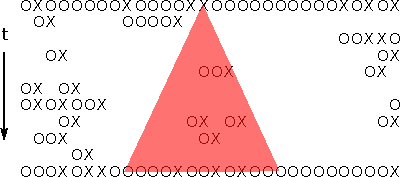
\includegraphics[width=\textwidth]{../../../writeup-plots/talk-tasep-fig-3}

    \end{column}
  \end{columns}

\end{frame}



% e^tG; previous work
\begin{frame}{Idealized solution}

  This is a continuous-time, finite-state Markov chain on length-$n$ sequences.
  
  \vspace{1em}

  Exact likelihood function, \\
  \hspace{2em} for observing sequnce $x$ evolve into $y$ in time $t$:
  \begin{align*}
    \P\{ X_t = y | X_0 = x \} = \left( e^{tG} \right)_{xy} .
  \end{align*}

  \vspace{1em}

  {\newthing Problem:} $G$ is a $4^n \times 4^n$ matrix.

\end{frame}


\begin{frame}{Previous work}

  \begin{itemize}

    \item Assume a $k$th order Markov model along the sequence \\
      -- Siepel \& Haussler 2003

    \item Expansion of $e^{tG}$ \\
      -- Lunter \& Hein 2004 

    \item Data augmentation: MCMC over true mutational path \\
      -- Hobolth 2008, Baele et al 2010

    \item various others

  \end{itemize}

\end{frame}

% Assumptions and not
\begin{frame}{Assumptions}

  We are assuming:
  \begin{itemize}

    \item homogeneity along the sequence

  \end{itemize}

  \vspace{2em}

  We are not assuming:
  \begin{itemize}

    \item stationarity

    \item reversibility

  \end{itemize}

  \vspace{2em}

  Example: GC-content need not be at equilibrium.

\end{frame}


%%%%%%%%% METHODS
\section{Statistical \& Computational Methods}

%   restrict to pattern frequencies: partial likelihood
\begin{frame}{Larger windows?}

  \begin{columns}[c]
    \begin{column}{.4\textwidth}

  First attempt:
  \begin{itemize}

    \item Pick a window size $w$

    \item Count all pairs of $w$-tuples: \\
      $n(a,b) = \# \{ a \to b \}$ \\
      {\aside (nonoverlapping?)}

    \item Compute $4^w \times 4^w$ transition matrix $G_w$.

  \end{itemize}

  \vspace{2em}

  Assume each $w$-window evolves indpendently --
  partial/pseudo-likelihood: 
  \begin{align*}
    \mathcal{L} = \prod_{a,b} n(a,b) \log \left( e^{tG_w} \right)_{ab} .
  \end{align*}

    \end{column}
    \begin{column}{.6\textwidth}

      Example: $w=3$
      \only<1>{
            {
          \begin{center} \setlength{\tabcolsep}{0pt} \begin{tabular}{cccccccccccccccccccccccccccccccccccccccccccccccccccccccccc}
            \cline{1-3}
            \tLL{C}&C&\tRR{C}&A&G&T&C&C&A&G&A&T&A&A&A&A&T&T&G&A&T&A&A&C&T&C\\
            \tLL{C}&A&\tRR{C}&A&G&T&C&C&A&G&A&T&A&A&A&A&T&C&G&A&T&A&A&C&T&C\\
            \cline{1-3}
          \end{tabular} \end{center} 
          }
      }
      \only<2>{
            {
          \begin{center} \setlength{\tabcolsep}{0pt} \begin{tabular}{cccccccccccccccccccccccccccccccccccccccccccccccccccccccccc}
            \cline{4-6}
            C&C&C&\tLL{A}&G&\tRR{T}&C&C&A&G&A&T&A&A&A&A&T&T&G&A&T&A&A&C&T&C\\
            C&A&C&\tLL{A}&G&\tRR{T}&C&C&A&G&A&T&A&A&A&A&T&C&G&A&T&A&A&C&T&C\\
            \cline{4-6}
          \end{tabular} \end{center} 
          }
      }
      \only<3>{
            {
          \begin{center} \setlength{\tabcolsep}{0pt} \begin{tabular}{cccccccccccccccccccccccccccccccccccccccccccccccccccccccccc}
            \cline{7-9}
            C&C&C&A&G&T&\tLL{C}&C&\tRR{A}&G&A&T&A&A&A&A&T&T&G&A&T&A&A&C&T&C\\
            C&A&C&A&G&T&\tLL{C}&C&\tRR{A}&G&A&T&A&A&A&A&T&C&G&A&T&A&A&C&T&C\\
            \cline{7-9}
          \end{tabular} \end{center} 
          }
      }

      \vspace{2em}

      {\struct but:} still misses edge effects.



    \end{column}
  \end{columns}
\end{frame}


%   still missing edge effects: marginalize over window
%     node average boundary
\begin{frame}{Still missing those edge effects}

  \begin{columns}[c]
    \begin{column}{.4\textwidth}

      {\newthing Solution:} Trim the bottom window.

      \vspace{1em}

      Count pairs of $(w,r)$-tuples, with $r<w$,

      \vspace{1em}

      computing the probability of a change by marginalizing over the omitted bases.

      \vspace{1em}

  Must still deal with nonindependence --
  partial/pseudo-likelihood: 
  \begin{align*}
    \mathcal{L} = \prod_{a,c} n(a,c) \sum_{b \supset c} \log \left( e^{tG_w} \right)_{ab} .
  \end{align*}

    \end{column}
    \begin{column}{.6\textwidth}

      Example: $w=3,r=1$
      \only<1>{
            {
          \begin{center} \setlength{\tabcolsep}{0pt} \begin{tabular}{cccccccccccccccccccccccccccccccccccccccccccccccccccccccccc}
            \cline{1-3}
            \tLL{C}&C&\tRR{C}&A&G&T&C&C&A&G&A&T&A&A&A&A&T&T&G&A&T&A&A&C&T&C\\
            \cline{1-1}\cline{3-3}
            C&\tLR{A}&C&A&G&T&C&C&A&G&A&T&A&A&A&A&T&C&G&A&T&A&A&C&T&C\\
            \cline{2-2}
          \end{tabular} \end{center} 
          }
      }
      \only<2>{
            {
          \begin{center} \setlength{\tabcolsep}{0pt} \begin{tabular}{cccccccccccccccccccccccccccccccccccccccccccccccccccccccccc}
            \cline{4-6}
            C&C&C&\tLL{A}&G&\tRR{T}&C&C&A&G&A&T&A&A&A&A&T&T&G&A&T&A&A&C&T&C\\
            \cline{4-4}\cline{6-6}
            C&A&C&A&\tLR{G}&T&C&C&A&G&A&T&A&A&A&A&T&C&G&A&T&A&A&C&T&C\\
            \cline{5-5}
          \end{tabular} \end{center} 
          }
      }
      \only<3>{
            {
          \begin{center} \setlength{\tabcolsep}{0pt} \begin{tabular}{cccccccccccccccccccccccccccccccccccccccccccccccccccccccccc}
            \cline{7-9}
            C&C&C&A&G&T&\tLL{C}&C&\tRR{A}&G&A&T&A&A&A&A&T&T&G&A&T&A&A&C&T&C\\
            \cline{7-7}\cline{9-9}
            C&A&C&A&G&T&C&\tLR{C}&A&G&A&T&A&A&A&A&T&C&G&A&T&A&A&C&T&C\\
            \cline{8-8}
          \end{tabular} \end{center} 
          }
      }

      {\struct Ex:} 
      \begin{align*}
        & \P\{\text{CCC} \to \cdot\text{A}\cdot\} = \\
        &\quad \P\{\text{CCC} \to \text{CAC} \} \\
        &\qquad {}+\P\{\text{CCC} \to \text{CAA} \}  \\
        &\qquad {}+\P\{\text{CCC} \to \text{CAG} \}  \\
        &\qquad {}+\P\{\text{CCC} \to \text{GAC} \}  \\
        &\qquad {}+\P\{\text{CCC} \to \text{GAT} \}  \\
        & \qquad {} + \cdots 
      \end{align*}



    \end{column}
  \end{columns}

\end{frame}


%   asymptotically correct: propagation of dependency
\begin{frame}{Asymptotic correctness}
  \begin{columns}[c]
    \begin{column}{.4\textwidth}

  {\struct Claim:} \\
  If the size of the trimmed window is large enough, this is a {\newthing correct} (partial) likelihood.

  \vspace{2em}

  {\struct ``Proof:''}
  The probability that a site has been affected by another more than $k$ bases away decays geometrically,

  \vspace{2em}

  so if $w-r$ is large enough, the number of sites for which we should have included information from sites outside $w$ is small.

    \end{column}
    \begin{column}{.6\textwidth}

      Ex: $w=8$ and $r=2$.

  \vspace{1em}

  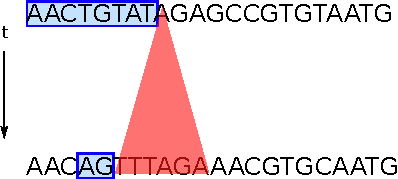
\includegraphics{../../../writeup-plots/talk-dependency-proof-fig}

    \end{column}
  \end{columns}

\end{frame}

%   likelihood function
\begin{frame}{Inference framework: recap}

  {\struct So far:} 
  can compute a partial likelihood for time series observations. \\
  (i.e.\ a single branch; total time confounded with overall mutation rate)

  \vspace{1em}

  {\struct Goal:} 
  Infer mutation rates, selection coefficients, time (confounded).

  \vspace{1em}

  {\struct Options:} \\
  \begin{itemize}

    \item Count patterns at all positions, \\
      do maximum likelihood \\
      $\longrightarrow$ uses all the data, faster

    \item Only count in nonoverlapping windows, \\
      add priors, MCMC \\
      $\longrightarrow$ obtains credible intervals

  \end{itemize}

  {\struct Questions:} \\
  \begin{itemize}

    \item How large a window $(w,r)$ is feasible?

    \item What about phylogenetics?

  \end{itemize}
  

\end{frame}

%   computation: sparse matrices
\begin{frame}{Computation: using sparseness}

  Likelihood requires, for $a \in \{A,C,G,T\}^w$ and $c \in \{A,C,G,T\}^r$,
  \[
  \sum_{b \supset c} \left( e^{tG} \right)_{ab} = ( \underset{\scriptstyle 4^w \times 4^w}{e^{tG}} \quad  \underset{\scriptstyle 4^w \times 4^r}{P} )_{ac} 
  \]
  where:
  \begin{itemize}
    \item $G$ is matrix of mutation rates --\\
      each row has $w$ nonzero entries if only single-base changes
    \item $P$ is projection matrix --\\
      each row has exactly one `1' .
  \end{itemize}

  {\struct Tools:} 
  \begin{itemize}

    \item Krylov methods for matrix exponentiation --\\
      evaluates $e^{tA} v$ with only 5--10 multiplications of a vector by $A$ \\
      {\aside (Sidje 1998; expm in R)}

    \item sparse matrix methods 
      {\aside (Matrix package in R)}

    \item efficient updating of $G$ with new parameters --\\
      nonzero entries are linear combinations of mutation rates.
    
  \end{itemize}

\end{frame}

%   phylogenetic peeling (?)
\begin{frame}{What about phylogenetics?}

  \begin{columns}[c]
    \begin{column}{.5\textwidth}

  If observations are on the tips of a tree, 
  add root frequencies to parameters,
  and peel towards tip with ``long'' observations:
  \begin{align*}
    M^1_{u,z} &= \pi_u \left( e^{t_C G} P \right)_{uz} \\
    M^2_{v,z} &= \sum_u \left( e^{t_{AB} G} \right)_{uv} M^1_{u,z} \\
    M^3_{v,y,z} &= \left( e^{t_B G} P \right)_{vy} M^2_{v,z} \\
    M^4_{x,y,z} &= \sum_v \left( e^{t_A G} P \right)_{vx} M^3_{v,y,z} \\
    \mathcal{L} &= \sum_{x,y,z} n(x,y,z) \log M^4_{x,y,z}
  \end{align*}

  \vspace{1em}

  {\newthing Note:} Need not use all $(x,y,z)$.

    \end{column}
    \begin{column}{.5\textwidth}

  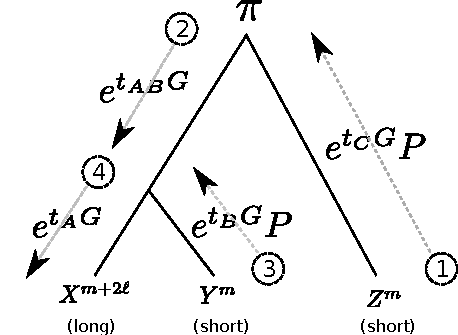
\includegraphics[width=\textwidth]{../../peeling-schematic}

  \vspace{2em}

  \begin{center}
  \small
  \begin{tabular}{cccc}
    $x$ & $y$ & $z$ & $n(x,y,z)$ \\
    \hline
    AAA & $\cdot$A$\cdot$ & $\cdot$A$\cdot$ & 1023 \\
    AAA & $\cdot$A$\cdot$ & $\cdot$C$\cdot$ & 42 \\
    AAA & $\cdot$C$\cdot$ & $\cdot$A$\cdot$ & 5  \\
    \vdots & \vdots & \vdots & \vdots 
  \end{tabular}
  \end{center}

    \end{column}
  \end{columns}

\end{frame}

\begin{frame}{Computation: upshot}

  $G$ is sparse and large; $e^{tG}$ is dense, and large -- \\
  \hspace{3em} but, only ever compute smaller dense matrices.

  \vspace{1em}

  {\struct Choices:}
  \begin{itemize}
    \item Long ($w$) and short ($r$) pattern sizes
    \item Set of short patterns: maximize information
  \end{itemize}

  \vspace{1em}

  {\struct Memory usage:} constant times the (pattern count) data.

  \vspace{1em}

  {\struct Computational time:} $O(w 4^{w} (\#\text{short patterns}))$ operations 
  \begin{itemize}
    \item $(w=5,r=1) \longrightarrow$  a second
    \item $(w=8,r=2) \longrightarrow$  a minute
  \end{itemize}

  \vspace{1em}

  {\struct Feasible:} window sizes, nearest neighbor context \\
  \hspace{3em} $w=4$: mean density of mutations ${} < 0.5$ per site\\
  \hspace{3em}   $w=8$: mean density of mutations ${} < 2$ per site

\end{frame}


%%%%%%%%% APPLICATIONS
\section{Applications}

\begin{frame}{Applications}

  Simulation:
  \begin{itemize}
    \item phylogenetics: single-base rates $+$ CpG 
    \item statistical physics: Ising model
  \end{itemize}

  \vspace{3em}

  Real data:
  \begin{itemize}
    \item now running
    \item \ldots ideas.
  \end{itemize}

\end{frame}

%   CpG
\begin{frame}{Nucleotide sequence: model}

  Simulated $10^6$ bases on a tree of length 1, \\
  with one branch twice as long as the other,\\
  equal base frequencies at the root,
  and mutation rates
  {\small
  \begin{center}
    \begin{tabular}{c@{\quad$\to$\quad}c@{\quad at rate\quad }c}
      $u$  &  $v$  &  $\mu$  \\
      \hline
       A & T   &  0.15  \\
       A & C   &  0.15  \\
       \vdots & \vdots & \vdots \\
       G & C &  0.15  \\
      CG   &  TG   &  0.45 \\
      CG   &  CA   &  0.45 
    \end{tabular}
  \end{center}
  }

  \vspace{2em}

  $\longrightarrow$ sequence divergence above 15\% $\longleftarrow$
  
  \vspace{2em}

  ({\struct note:} CpG rate is 5--30 times background rate\ldots\\
  \hspace{3em} but, not modeling methylation.)

\end{frame}

\begin{frame}{Nucleotide sequence: results}

  Priors on the 17 parameters; MCMC to get posterior distribution;\\
  \hspace{2em} length-two windows: $w=5$ and $r=1$

  \begin{center}
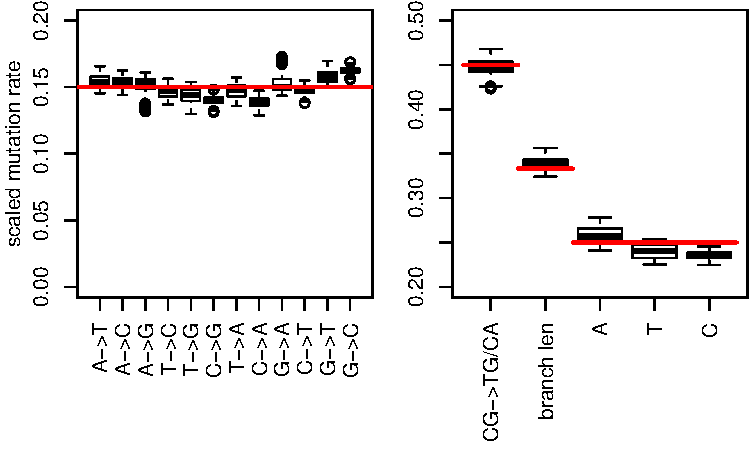
\includegraphics[width=\textwidth]{../../../writeup-plots/selsims-2013-06-03-13-17-0187525-estimate-boxplots}
\end{center}

\end{frame}

%   Ising
\begin{frame}{Statistical physics: model}

  Ising model, with Glauber dynamics: \\
  \hspace{2em} sites are $\pm $ ``magnetic dipoles''; \\
  \hspace{2em}   energy of a configuration $x$ is $s(x) = - \beta \sum_i x_i x_{i+1} - \gamma \sum_i x_i$; \\
   \hspace{2em}  local perturbations resolve proportional to $e^{-\Delta s}$

   \vspace{2em}

   Mutations: $(+ \to -)$ and $(- \to +)$ at rate 1

   \vspace{2em}

  Selection: probability of fixation $f(s) = 1/(1+e^{-s})$, \\
  \hspace{3em} ``selection'' coefficients
  \begin{center}
    \begin{tabular}{c|c}
      $u$  &  $s(u)$ \\
      \hline
      $+$ & $+\gamma$ \\
      $-$ & $-\gamma$ \\
      $--$, $++$  & $+\beta$ \\
      $-+$, $+-$  & $-\beta$ 
    \end{tabular}
  \end{center}

\end{frame}


\begin{frame}{Statistical physics: results}
  \begin{columns}[c]
    \begin{column}{.4\textwidth}

      With $\lambda = \beta = \gamma = 1$ and $t = 0.1$  ($\approx$ 13\% sites differ), $10^6$ sites; \\

      \vspace{1em}

      $w=9$ and $r=3$;

      \vspace{1em}

      MCMC over posterior distribution:


    \end{column}
    \begin{column}{.6\textwidth}

  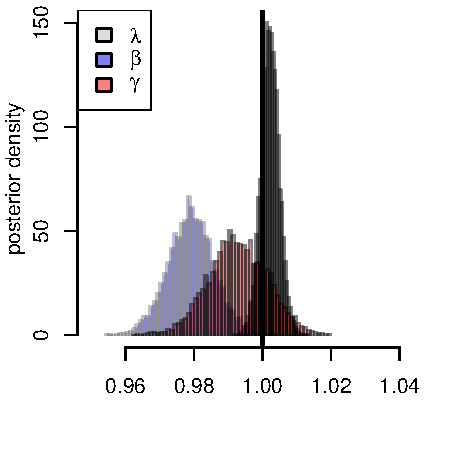
\includegraphics[width=\textwidth]{../../../writeup-plots/selsims-2013-05-28-17-12-0275615-estimate-hists}

    \end{column}
  \end{columns}

\end{frame}

%   real data?
\begin{frame}{Real data}

  still running\ldots

\end{frame}

%   ancestral state reconstruction
\begin{frame}{Other applications}

  Ancestral state reconstruction \\
  \hspace{2em} deep in the tree
    
  \vspace{3em}

  Ancestral methylation inference\\
  \hspace{2em} CG $\to$ TG or CA rate depends on methylation state \\
  \hspace{2em} \ldots so branch-specific mutation rate infers methylation
    
  \vspace{3em}

  Context-dependent effects:\\
  \hspace{2em} transcription or repair machinery effects? \\
  \hspace{2em} {\aside (recently, Harris \& Nielsen 2013; Schrider et al 2011; Terekhanova et al 2013)}

\end{frame}

%%%%% ok all done
\begin{frame}{Conclusions}

  On nucleotide sequence, it is currently feasible to rigorously
  \begin{itemize}

    \item identify short-range context-dependent effects ($\le 9$ bases) \\
      across high levels of sequence divergence \\

    \item root trees 
      
    \item infer nonstationary mutation processes and sequence content

  \end{itemize}
  
  \vspace{2em}

  Drawbacks:
  \begin{itemize}

    \item doesn't model sitewise variable mutation rates 

    \item becomes slow for long context windows (but, parallelizable)

  \end{itemize}
  
  \vspace{2em}

  (Almost) available as an {\texttt R} package.

\end{frame}

\begin{frame}{Thanks}

  Matt Dean
  
  Rasmus Nielsen

  Simon Tavar\'e

  Graham Coop

  Sergey Nudzhin

\end{frame}

\end{document}
